%% This is an example first chapter.  You should put chapter/appendix that you
%% write into a separate file, and add a line \include{yourfilename} to
%% main.tex, where `yourfilename.tex' is the name of the chapter/appendix file.
%% You can process specific files by typing their names in at the 
%% \files=
%% prompt when you run the file main.tex through LaTeX.
\chapter{Simulation Results}

\section{Benchmark Studies}

\colorlet{color0ms}{blue}
\colorlet{color50ms}{OliveGreen}
\colorlet{color100ms}{RawSienna}
\colorlet{color200ms}{Magenta}
\colorlet{color300ms}{Orange}

\newcommand{\threec}[3]{\ensuremath{\textcolor{color0ms}{#1}|\textcolor{color50ms}{#2}|\textcolor{color100ms}{#3}}}

\newcommand{\fivec}[5]{\begin{centering}\ensuremath{\hspace{0.7em}\textcolor{color0ms}{#1}|\textcolor{color50ms}{#2} \newline \hspace{-5em} \textcolor{color100ms}{#3}|\textcolor{color200ms}{#4}|\textcolor{color300ms}{#5}}\end{centering}}

\newcommand{\fivecfordeadlock}[5]{\begin{centering}\ensuremath{\hspace{0.55em}\textcolor{color0ms}{#1}|\textcolor{color50ms}{#2} \newline \hspace{-5em} \textcolor{color100ms}{#3}|\textcolor{color200ms}{#4}|\textcolor{color300ms}{#5}}\end{centering}}

\newcommand{\threecb}[3]{\ensuremath{\textcolor{color0ms}{\textbf{#1}}|\textcolor{color50ms}{\textbf{#2}}|\textcolor{color100ms}{\textbf{#3}}}}
\newcommand{\fivecb}[5]{\begin{centering}\ensuremath{\hspace{0.7em}\textcolor{color0ms}{\textbf{#1}}|\textcolor{color50ms}{\textbf{#2}} \newline \textcolor{color100ms}{\textbf{#3}}|\textcolor{color200ms}{\textbf{#4}}|\textcolor{color300ms}{\textbf{#5}}}\end{centering}}

% \begin{table*}[!h]
%     \renewcommand{\arraystretch}{2}
%     \caption{\centering Benchmark Studies: Cases \textcolor{color0ms}{$\delayIntroduced{}=0$~ms}, \textcolor{color50ms}{$\delayIntroduced{}=50$~ms}, \textcolor{color100ms}{$\delayIntroduced{}=100$~ms}, \textcolor{color200ms}{$\delayIntroduced{}=200$~ms}, and \textcolor{color300ms}{$\delayIntroduced{}=300$~ms}.}
%     \label{tab:sim_compare}    
%     % \renewcommand{\arraystretch}{1.6}
%     \centering
%     \resizebox{\textwidth}{!}{
%     \setlength{\tabcolsep}{6pt}
%     \begin{tabular}{>{\centering\arraybackslash}m{0.07\textwidth}|>{\centering\arraybackslash}m{0.05\textwidth}|>{\centering\arraybackslash}m{0.08\textwidth}|>{\centering\arraybackslash}m{0.08\textwidth}|>{\centering\arraybackslash}m{0.06\textwidth}|>{\centering\arraybackslash}m{0.12\textwidth}|>{\centering\arraybackslash}m{0.14\textwidth}|>{\centering\arraybackslash}m{0.2\textwidth}|>{\centering\arraybackslash}m{0.12\textwidth}|>{\centering\arraybackslash}m{0.14\textwidth}}
%         \toprule
%         \centering Method & \centering Async.? & \centering \delayParameter{} [ms] & \centering Collision-free rate [\%] & Deadlock rate [\%] & \centering Avg number \\ of stops & \centering \intaccelsquared{} [\SI{}{\m^2/\s^3}] & \centering \intjerksquared{} [\SI{}{\m^2/\s^5}] & \centering Avg Travel Time [s] & \centering Avg Travel Distance [m] \tabularnewline
%         \hline \hline

%         %% RMADER
%         \RMADER{} & \YesGreen & \fivec{75}{125}{175}{275}{375} & \fivecb{100}{100}{100}{100}{100} & \fivecfordeadlock{1}{1}{0}{0}{0} & \fivec{0.07}{0.188}{0.314}{0.425}{0.781} & \fivec{217.05}{230.02}{245.36}{268.64}{277.2} & \fivec{2191.8}{2638.3}{3002.5}{3685.1}{4205.07} & \fivec{10.6}{11.3}{12.7}{12.85}{15.56} & \fivec{20.3}{20.5}{20.5}{20.6}{20.7} \tabularnewline
%         \hline

%         %% WOCHECKRMADER
%         \WOCHECKRMADER{} & \YesGreen & \fivec{75}{125}{175}{275}{375} & \fivecb{100}{100}{100}{100}{100} & \fivecfordeadlock{0}{2}{3}{0}{5} & \fivec{0.192}{0.304}{0.399}{0.572}{0.95} & \fivec{228.9}{243.9}{259.6}{291.43}{296.16} & \fivec{2774.5}{3219.4}{3576.5}{4477.77}{5079.93} & \fivec{14.9}{16.4}{12.8}{14.26}{18.58} & \fivec{20.5}{20.7}{20.7}{21.0}{21.2} \tabularnewline
%         \hline

%         %% MADER
%         \MADER{} & \YesGreen & N/A & \fivecb{95}{92}{87}{72}{70} & \fivecfordeadlock{0}{0}{0}{0}{0} & \fivec{0.001}{0.006}{0.009}{0.004}{0.009} & \fivec{63.0}{61.6}{61.9}{62.8}{62.6} & \fivec{765.9}{761.6}{761.2}{769.0}{750.6} & \fivec{8.2}{9.1}{9.2}{9.3}{8.6} & \fivec{20.5}{20.5}{20.5}{20.5}{20.5} \tabularnewline
%         \hline

%         %% EGO-Swarm
%         \EGOswarm{} & \YesGreen & N/A & \fivecb{34}{27}{27}{48}{29} & \fivecfordeadlock{0}{0}{0}{0}{0} & \fivec{0.058}{0.057}{0.048}{0.051}{0.057} & \fivec{908.5}{948.4}{941.9}{876.4}{930.9} & \fivec{118068.3}{130966.9}{120610.8}{107619.2}{108491.9} & \fivec{5.3}{5.3}{5.4}{5.4}{5.4} & \fivec{30.8}{31.0}{30.9}{31.0}{31.0}   \tabularnewline
%         \hline

%         %% EDG-Team
%         \EDGteam{} & \YesGreen/\NoRed & N/A & \fivecb{100}{100}{99}{99}{99} & \fivec{0}{0}{0}{0}{0} & \fivec{0.176}{0.162}{0.179}{0.181}{0.191} & \fivec{224.6}{227.5}{222.2}{226.4}{225.6} & \fivecfordeadlock{4877.5}{5739.2}{5095.2}{5765.9}{5800.8} & \fivec{13.6}{13.9}{15.2}{15.2}{15.4} & \fivec{31.4}{31.4}{31.3}{31.3}{31.2}  \tabularnewline
%         \bottomrule 
%     \end{tabular}
%     }
% \end{table*}

% \begin{table*}[!h]
%     \renewcommand{\arraystretch}{2}
%     \caption{\centering Benchmark Study Case 1 $\delayIntroduced{}=0$~ms}
%     \label{tab:sim_compare}    
%     % \renewcommand{\arraystretch}{1.6}
%     \centering
%     \resizebox{\textwidth}{!}{
%     \setlength{\tabcolsep}{6pt}
%     \begin{tabular}{>{\centering\arraybackslash}m{0.07\textwidth}|>{\centering\arraybackslash}m{0.05\textwidth}|>{\centering\arraybackslash}m{0.08\textwidth}|>{\centering\arraybackslash}m{0.08\textwidth}|>{\centering\arraybackslash}m{0.06\textwidth}|>{\centering\arraybackslash}m{0.12\textwidth}|>{\centering\arraybackslash}m{0.14\textwidth}|>{\centering\arraybackslash}m{0.2\textwidth}|>{\centering\arraybackslash}m{0.12\textwidth}|>{\centering\arraybackslash}m{0.14\textwidth}}
%         \toprule
%         \centering Method & \centering Async.? & \centering \delayParameter{} [ms] & \centering Collision-free rate [\%] & Deadlock rate [\%] & \centering Avg number \\ of stops & \centering \intaccelsquared{} [\SI{}{\m^2/\s^3}] & \centering \intjerksquared{} [\SI{}{\m^2/\s^5}] & \centering Avg Travel Time [s] & \centering Avg Travel Distance [m] \tabularnewline
%         \hline \hline

%         %% RMADER
%         \RMADER{} & \YesGreen & 75 & 100 & 1 & 0.07 & 217.05 & 2191.8 & 10.6 & 20.3 \tabularnewline
%         \hline

%         %% WOCHECKRMADER
%         \WOCHECKRMADER{} & \YesGreen & 75 & 100 & 0 & 0.192 & 228.9 & 2774.5 & 14.9 & 20.5 21.2  \tabularnewline
%         \hline

%         %% MADER
%         \MADER{} & \YesGreen & N/A & 95 & 0 & 0.001 & 63.0 & 765.9 & 8.2 & 20.5 \tabularnewline
%         \hline

%         %% EGO-Swarm
%         \EGOswarm{} & \YesGreen & N/A & 34 & 0 & 0.058 & 908.5 & 118068.3 & 5.3 & 30.8 \tabularnewline
%         \hline

%         %% EDG-Team
%         \EDGteam{} & \YesGreen/\NoRed & N/A & 100 & 0 & 0.176 & 224.6 & 4877.5 & 13.6 & 31.4 \tabularnewline
%         \bottomrule 
%     \end{tabular}
%     }
% \end{table*}

\begin{figure}
    \centering
    \subcaptionbox{For Agent~J, the colored trajectory is the committed (safety-guaranteed) trajectory (\trajJ{}), and the grey trajectory is the newly optimized trajectory (\trajJNew{}).\label{fig:circle_traj_new}}{
    \begin{tikzpicture}[every text node part/.style={align=center}]
    \node {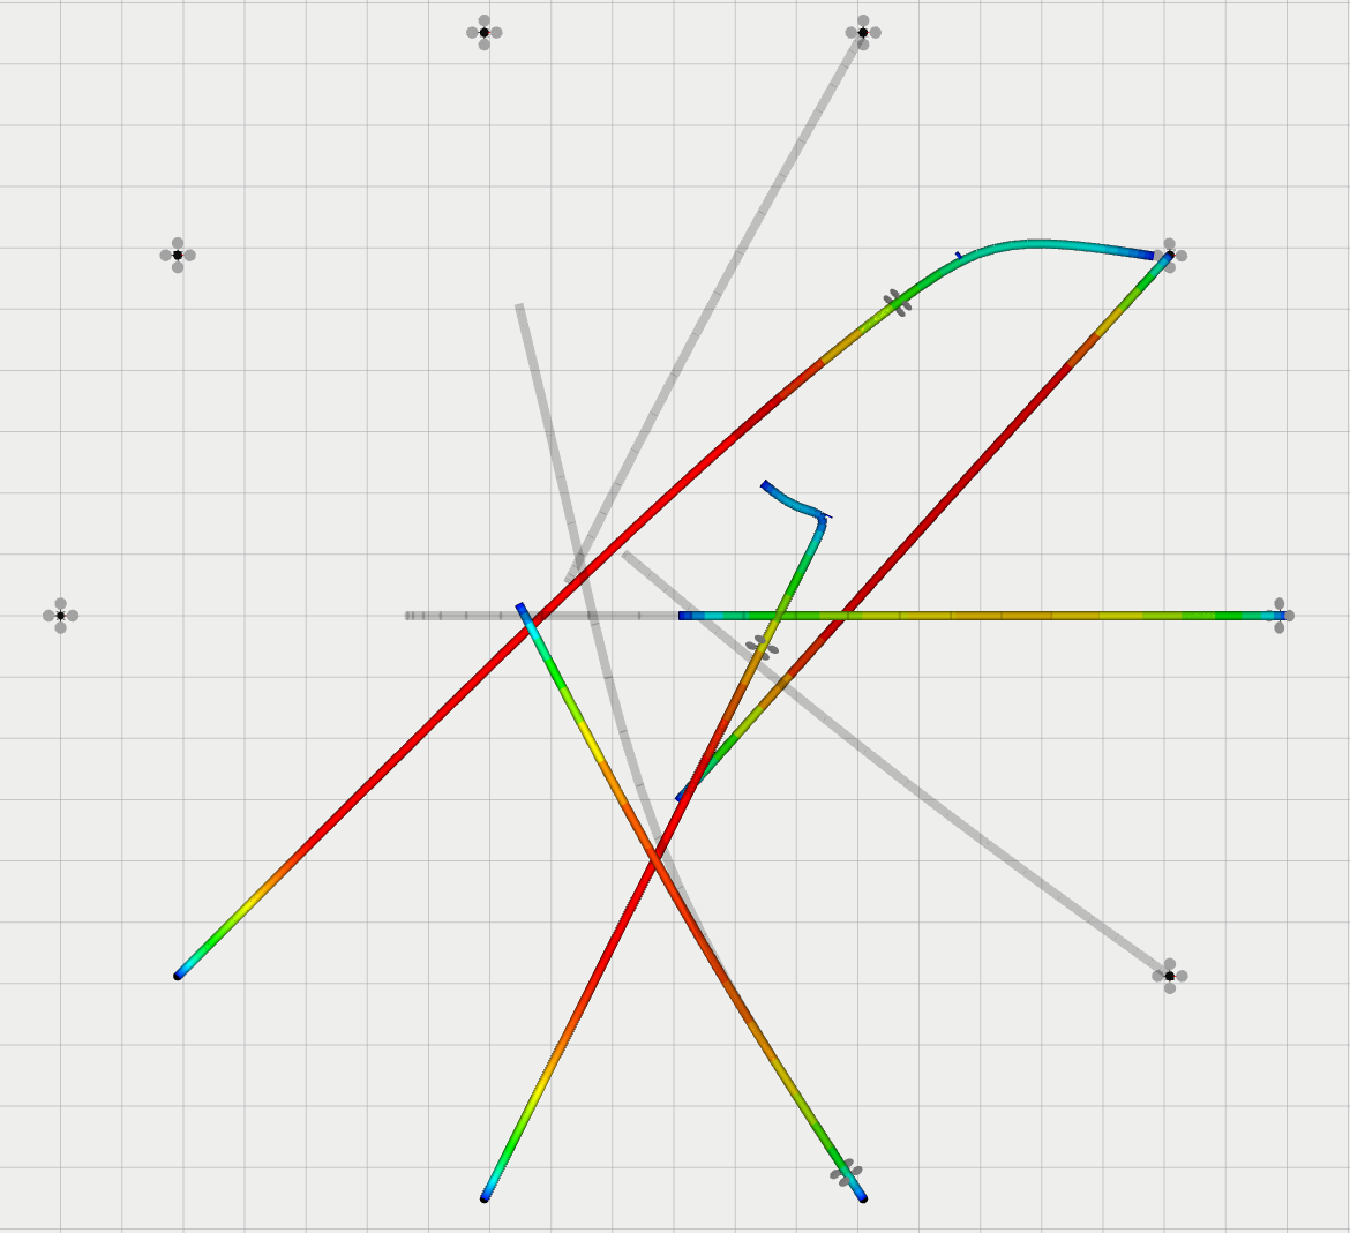
\includegraphics[width=0.45\columnwidth]{figures/rmader_two_traj_explained.pdf}};
    \node [rectangle] at (1.2, -1.6) {\scriptsize Agent J};
    \node [circle, draw] (c) at (0.5,-1.6){};
    \node (trajjnew) [rectangle] at (-1.2, 1.2) {\scriptsize \trajJNew{} (grey)}; 
    \draw [-stealth] (trajjnew) -- (-0.4, 0.4);
    \node (trajj) [rectangle] at (-1.2, -1) {\scriptsize \trajJ{} (colored)}; 
    \draw [-stealth] (trajj) -- (-0.38, -0.4);
    \end{tikzpicture}}
    \subcaptionbox{Actual trajectories flown by the agents. All 10 agents successfully swap their positions in a circle configuration. Agent J reached the goal.\label{fig:circle_traj_history}}{
    \begin{tikzpicture}[every text node part/.style={align=center}]
    \node {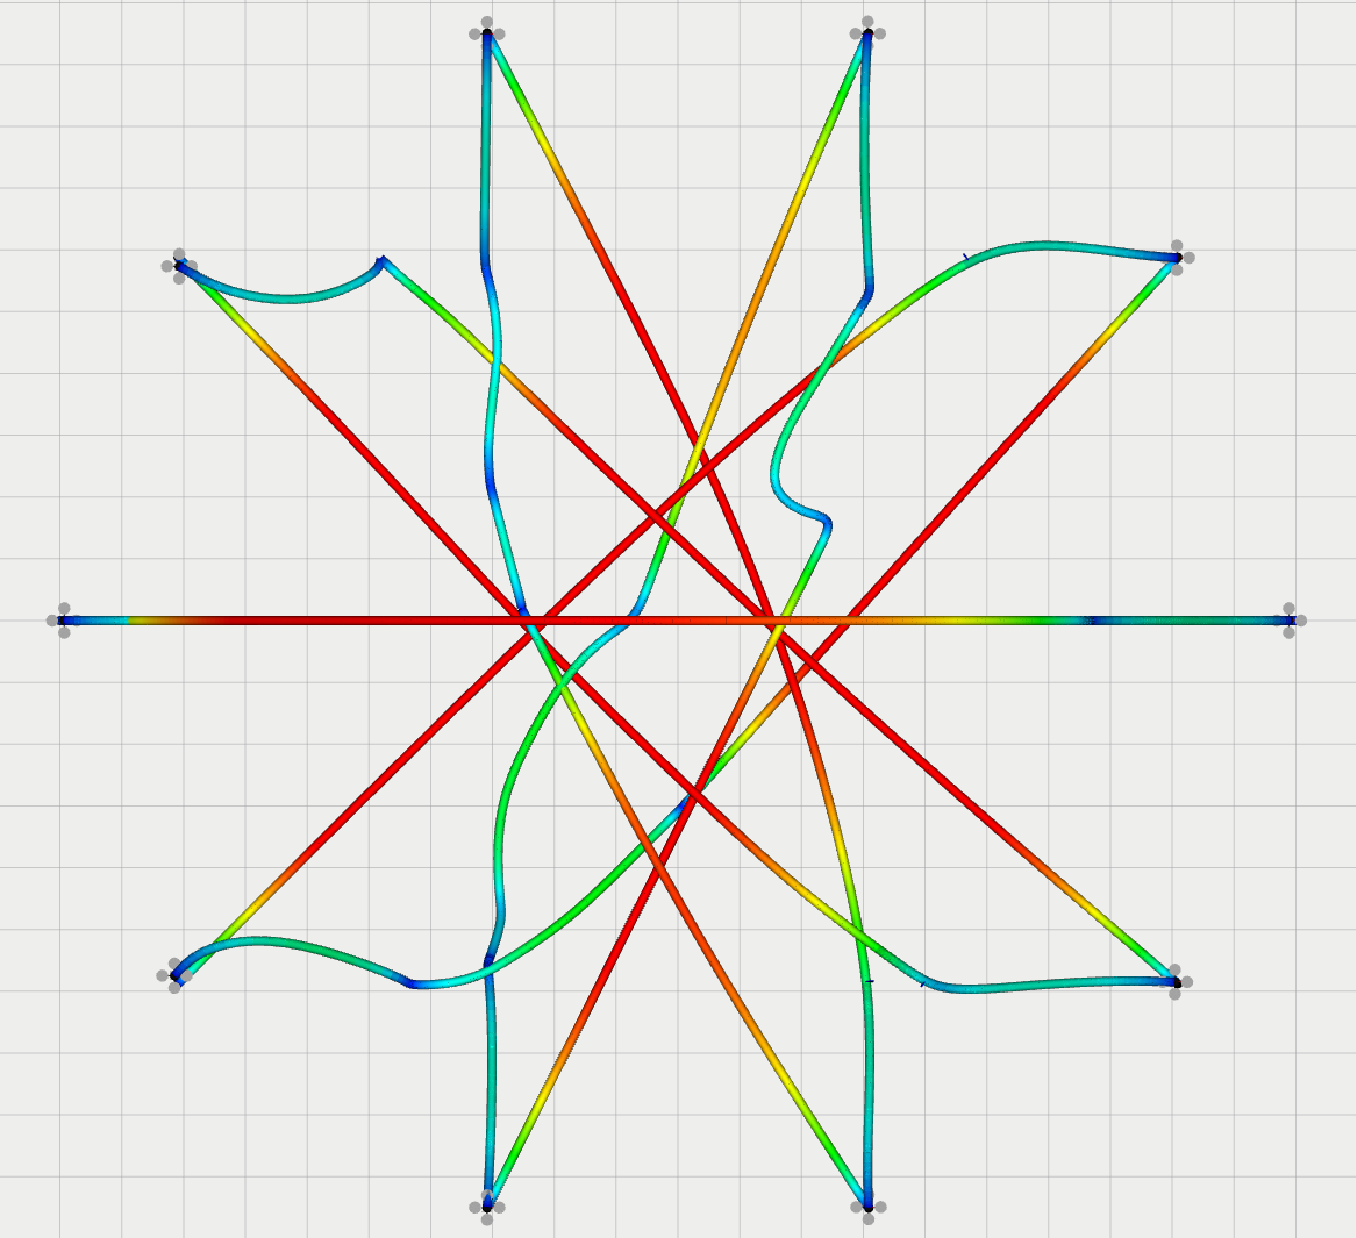
\includegraphics[width=0.45\columnwidth]{figures/rmader_two_traj_explained_finished.pdf}};
    \node [rectangle] at (-1.2, 1.6) {\scriptsize Agent J};
    \node [circle, draw] (c) at (-0.55,1.6){};
    \end{tikzpicture}}
    \caption{10 agents employing RMADER exchange their positions in a circle of radius \SI{20}{\m}. In the colored trajectories, red represents a high speed while blue denotes a low speed.}
    \label{fig:rmader_sim1}
\end{figure}

% \begin{figure*}
%     \begin{tabular}{ccc}
%       \subfloat[\centering Collision-free Trajectory Rate \label{fig:sim_collision_free_traj_rate}]{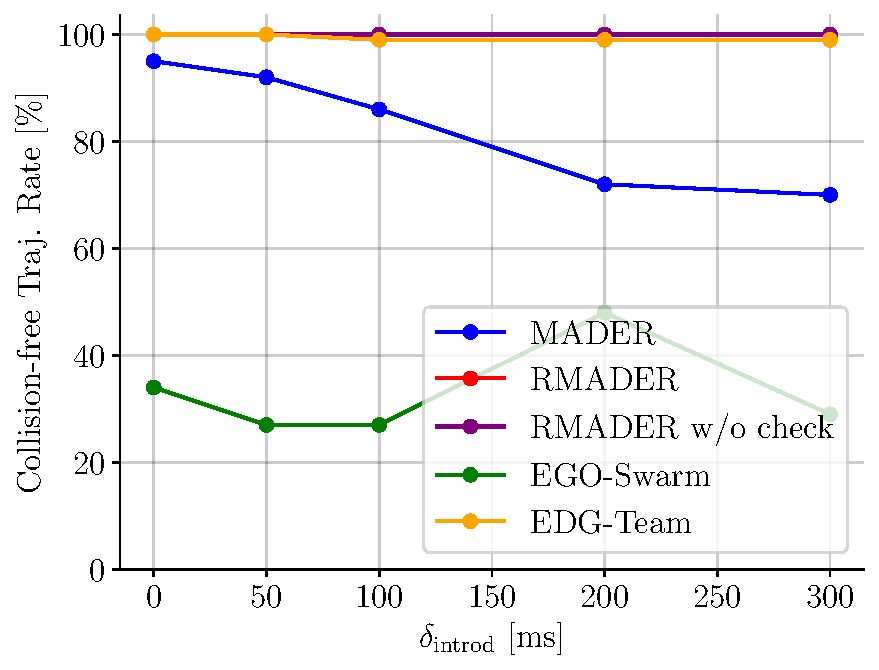
\includegraphics[width=0.3\textwidth]{figures/collision_free_traj.pdf}} &
%       \subfloat[\centering Avg. Travel Time\label{fig:sim_completion_time}]{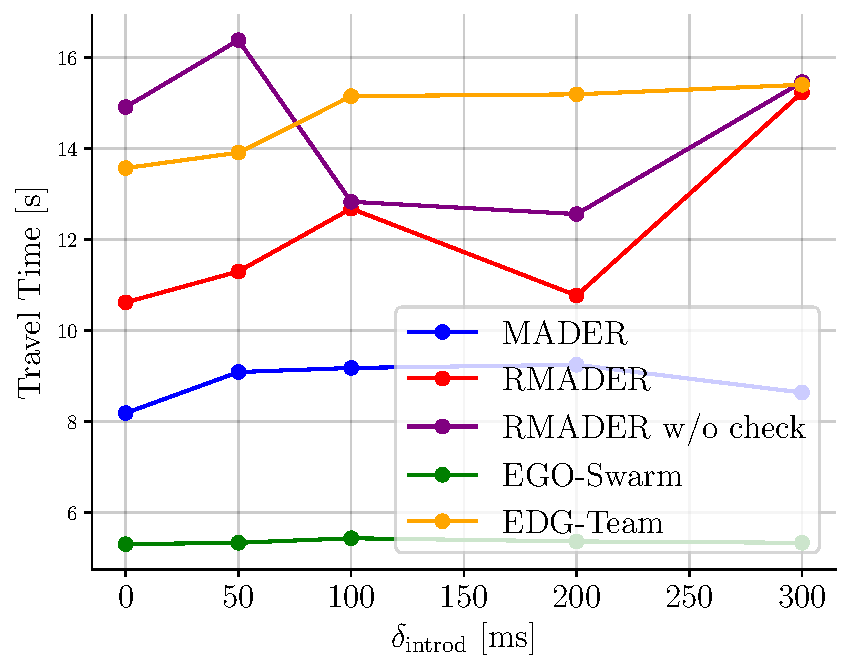
\includegraphics[width=0.3\textwidth]{figures/travel_time.pdf}} &
%       \subfloat[\centering Number of Stops \label{fig:sim_traj_smooth_acc}]{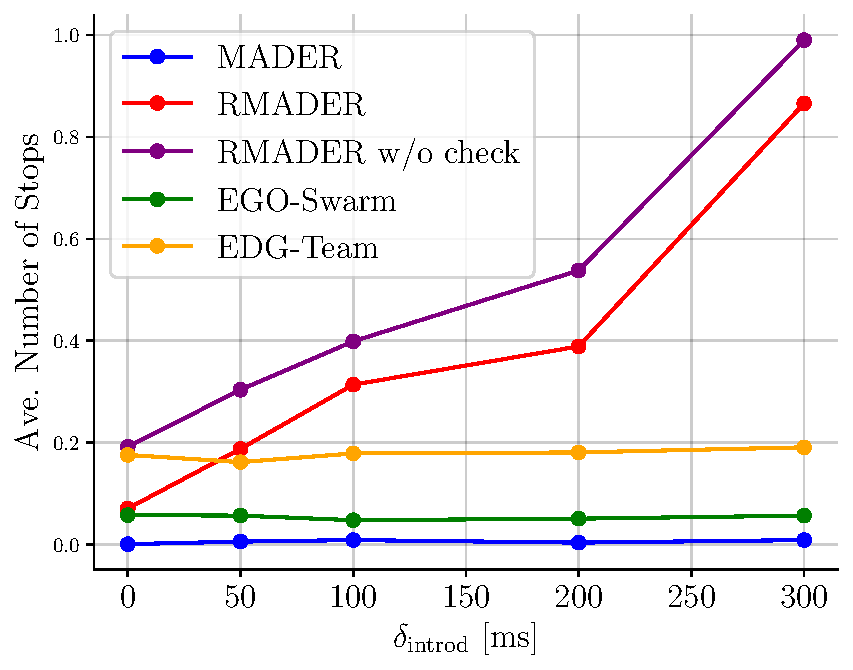
\includegraphics[width=0.3\textwidth]{figures/stop.pdf}} \\
%       \subfloat[\centering Trajectory Smoothness (Acceleration) \label{fig:sim_traj_smooth_acc}]{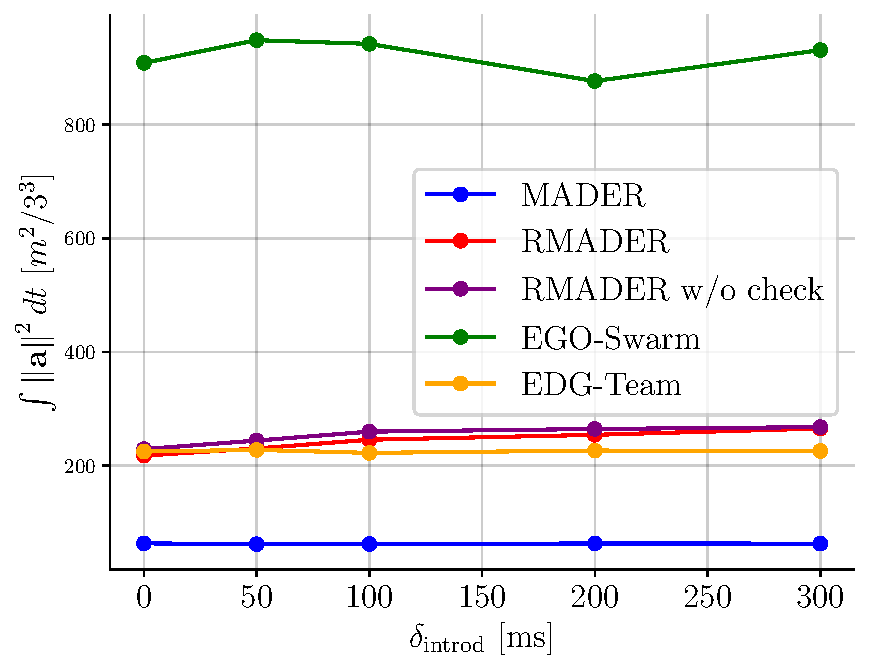
\includegraphics[width=0.3\textwidth]{figures/traj_smoothness_acc.pdf}} &
%       \subfloat[\centering Trajectory Smoothness (Jerk) \label{fig:sim_traj_smooth_jer}]{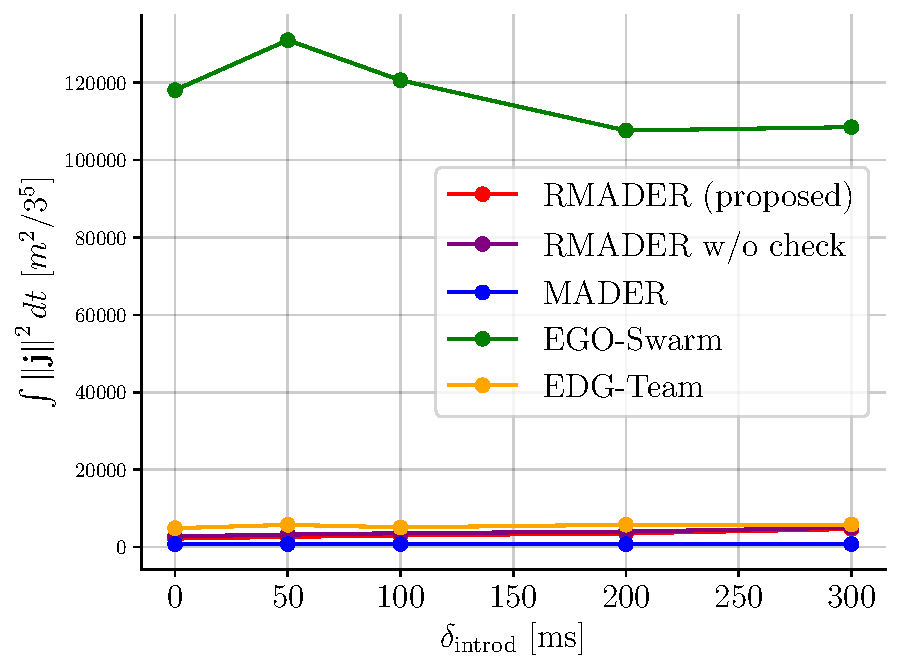
\includegraphics[width=0.3\textwidth]{figures/traj_smoothness_jer.pdf}} &
%       \subfloat[\centering Average total travel distance per agent\label{fig:sim_total_travel_dist}]{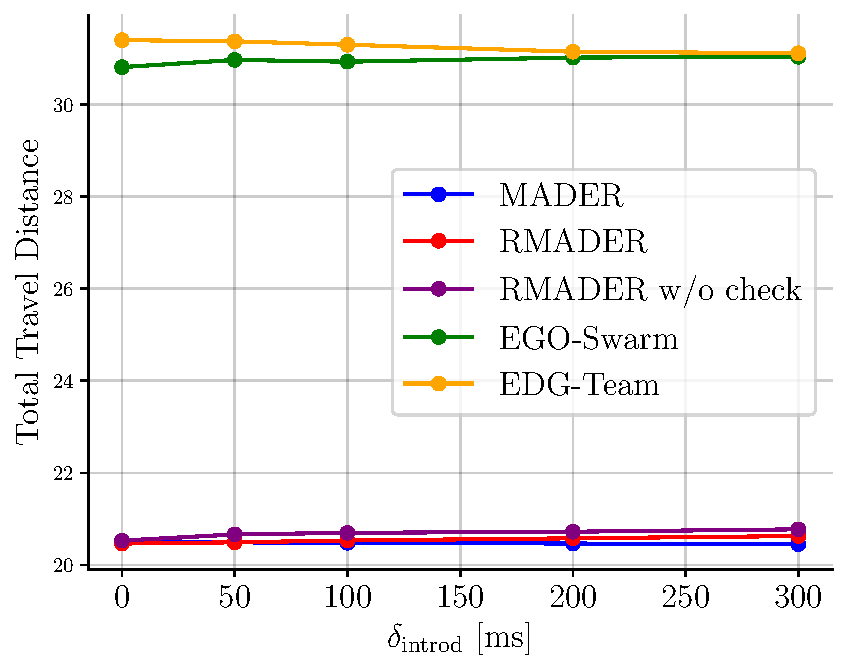
\includegraphics[width=0.3\textwidth]{figures/total_dist.pdf}}
%     \end{tabular}
%     \caption{100 Flight Simulation Results: Fig.~\ref{fig:sim_collision_free_traj_rate} shows RMADER generates collision-free trajectory at 100\%, while other state-of-the-art approaches fail when communication delays are introduced. 
%     To maintain collision-free trajectory generation, RMADER periodically occupies two trajectories, and other agents need to consider two trajectories as a constraint, which could lead to conservative plans - longer \emph{Travel Time} and more \emph{Avg. Number of Stops}. 
%     This is a trade-off between safety and performance. MADER reports a few collided trajectory because \delayActual{} $>$ \SI{0}{\ms}. These figures are slightly different from the ones presented in \cite{kondo2022robust} - we believe the reasons are (1) RMADER's parameters are extensively tuned, (2) to introduce artificial communication delays efficiently, we improved the code for all the methods, (3) simulations with multiagent planners are stochastic.} 
%     \label{fig:sim_simulation_summary}
% \end{figure*}

\begin{figure*}
    \centering
    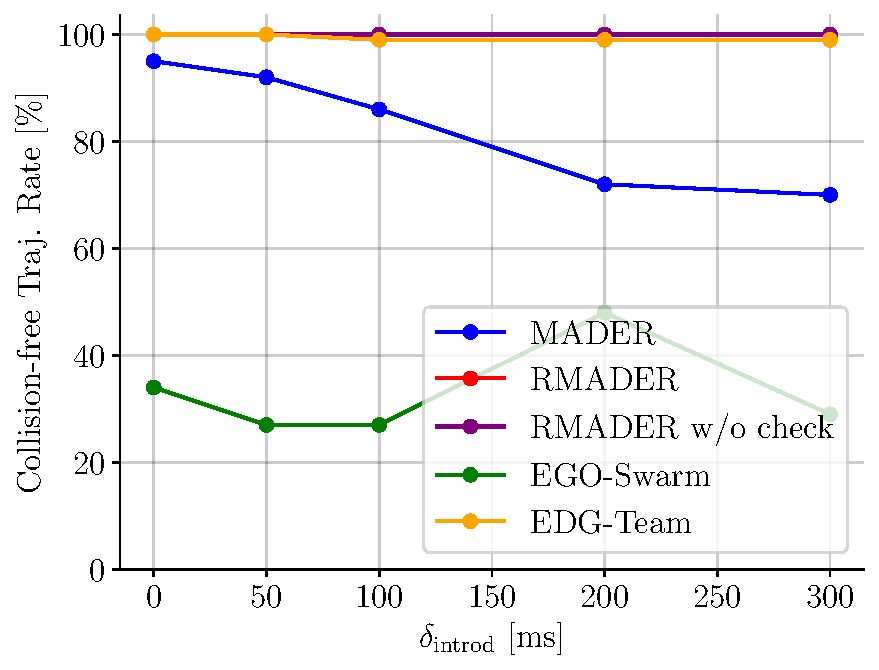
\includegraphics[width=0.6\textwidth]{figures/collision_free_traj.pdf}
    \caption{\centering Collision-free Trajectory Rate}
    \label{fig:sim_collision_free_traj_rate}
\end{figure*}

\begin{figure*}
    \centering
    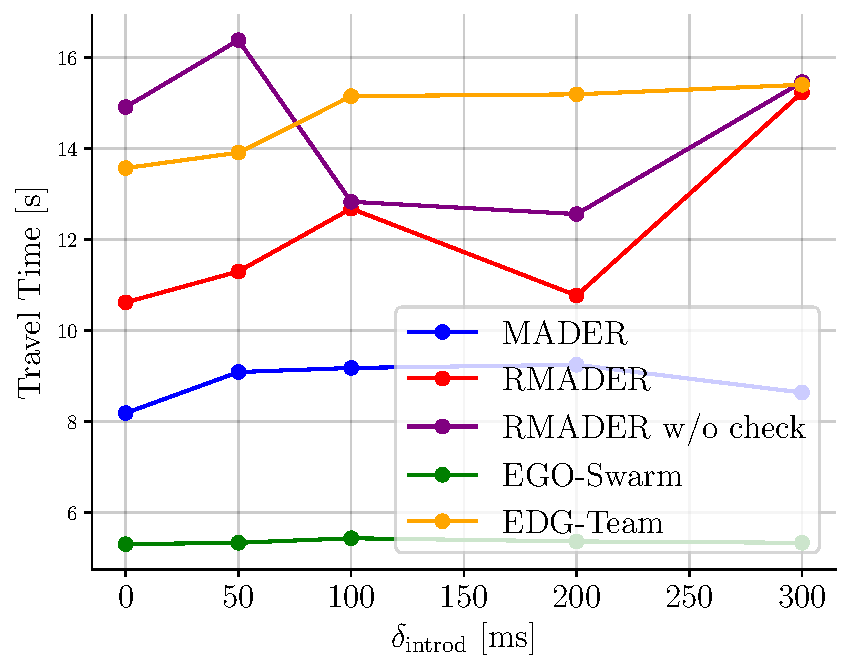
\includegraphics[width=0.6\textwidth]{figures/travel_time.pdf}
    \caption{\centering Avg. Travel Time}
    \label{fig:sim_travel_time}
\end{figure*}

\begin{figure*}
    \centering
    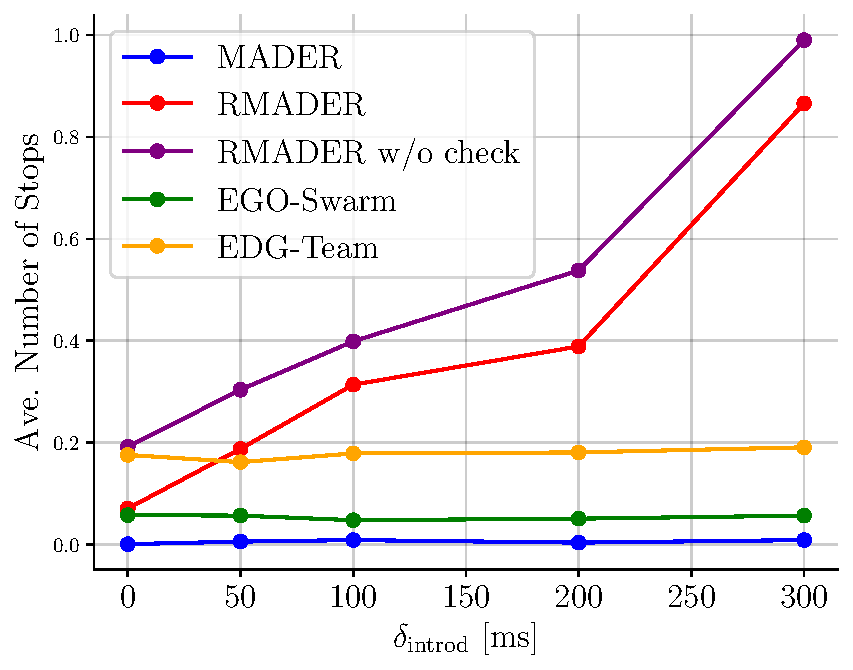
\includegraphics[width=0.6\textwidth]{figures/stop.pdf}
    \caption{\centering Number of Stops}
    \label{fig:sim_stop}
\end{figure*}

\begin{figure*}
    \centering
    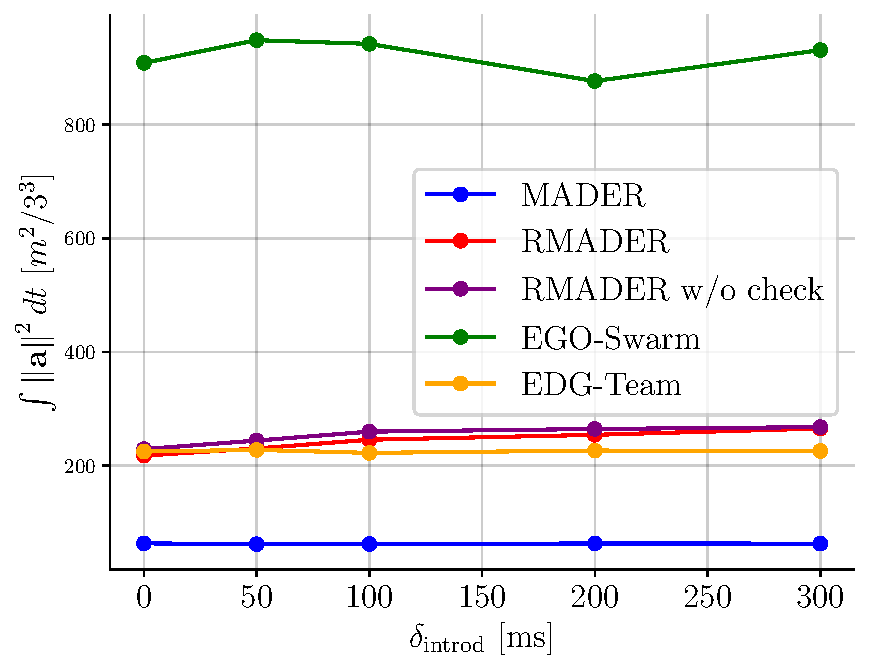
\includegraphics[width=0.6\textwidth]{figures/traj_smoothness_acc.pdf}
    \caption{\centering Average total travel distance per agent}
    \label{fig:traj_smoothness_acc}
\end{figure*}

\begin{figure*}
    \centering
    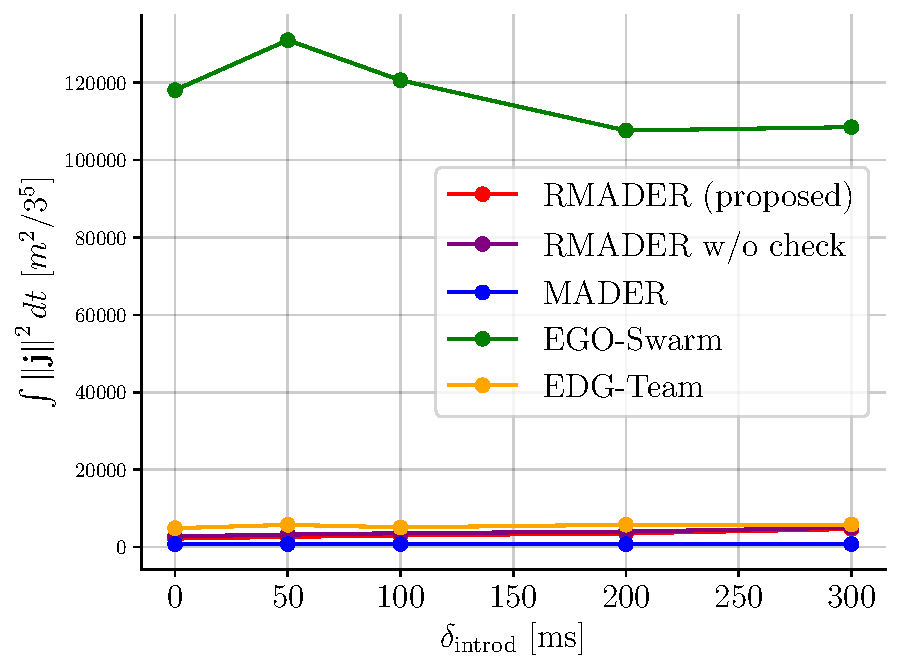
\includegraphics[width=0.6\textwidth]{figures/traj_smoothness_jer.pdf}
    \caption{\centering Trajectory Smoothness (Jerk)}
    \label{fig:traj_smoothness_jerk}
\end{figure*}

\begin{figure*}
    \centering
    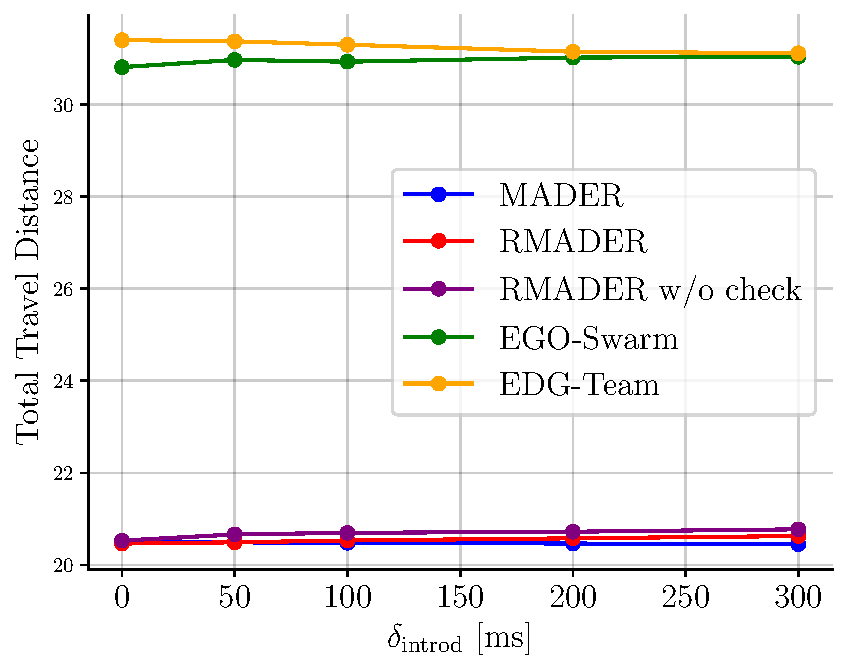
\includegraphics[width=0.6\textwidth]{figures/total_dist.pdf}
    \caption{\centering Average total travel distance per agent}
    \label{fig:total_dist}
\end{figure*}

100 Flight Simulation Results: Fig.~\ref{fig:sim_collision_free_traj_rate} shows RMADER generates collision-free trajectory at 100\%, while other state-of-the-art approaches fail when communication delays are introduced. 
    To maintain collision-free trajectory generation, RMADER periodically occupies two trajectories, and other agents need to consider two trajectories as a constraint, which could lead to conservative plans - longer \emph{Travel Time} and more \emph{Avg. Number of Stops}. 
    This is a trade-off between safety and performance. MADER reports a few collided trajectory because \delayActual{} $>$ \SI{0}{\ms}. These figures are slightly different from the ones presented in \cite{kondo2022robust} - we believe the reasons are (1) RMADER's parameters are extensively tuned, (2) to introduce artificial communication delays efficiently, we improved the code for all the methods, (3) simulations with multiagent planners are stochastic.

We tested EGO-Swarm~\cite{zhou_ego-swarm_2020}, EDT-Team~\cite{hou_enhanced_2022}, MADER~\cite{tordesillas_mader_2022}, RMADER, and RMADER without Check, on a \texttt{Lambda} computer with AMD Threadripper 3960X 24-Core, 48-Thread. 
For each algorithm, we introduced $0$, $50$, $100$, $200$, and \SI{300}{\ms} communication delay into every message exchanged among agents. 
We then conducted \textbf{100 simulations} with 10 agents positioned in a \SI{10}{\m} radius circle, exchanging positions diagonally as shown in Fig.~\ref{fig:rmader_sim1}.
Note that we used the convex MADER presented in \cite{kondo2022robust} for MADER, RMADER, and RMADER without Check.
The maximum dynamic limits are set to \SI{10}{\m/\s}, \SI{20}{\m/\s^2}, and \SI{30}{\m/\s^3} (velocity, acceleration, and jerk, respectively).
EGO-Swarm and EDG-Team carry out a sequential startup \textemdash agents commit their first trajectory in a pre-determined order to avoid initial trajectory conflicts, and therefore we also introduced \SI{0.25}{\second}-apart startup into MADER and RMADER. 

Table~\ref{tab:sim_compare} and Fig.~\ref{fig:sim_simulation_summary} showcase each approach's performance in simulations. 
When \NeccessaryCond{} holds, collision-free trajectory planning is guaranteed, and therefore RMADER generates \textbf{0 collisions} for all the \delayIntroduced{}, while other approaches suffer collisions. 
As expected, the longer \delayIntroduced{} more collisions EGO-Swarm, EDG-Team, and MADER generate.

It is also worth mentioning that RMADER's robustness to communication delays is obtained by layers of conflict checks and agents periodically holding two trajectories, which can result in generating conservative trajectories and trading off UAV performance. 
For instance, \emph{Avg. Number of Stops} in Table~\ref{tab:sim_compare}, suggests more stoppage than other approaches, and although RMADER reports no collisions, it suffers a small number of deadlocks.

\section{Simulations with Dynamic Obstacles}

To verify RMADER's robustness to dynamic environments, we performed 100 simulations with 10 agents with 10 dynamic obstacles under \SI{50}{\ms} communication delays and compare its performance to MADER. The agents' size is \qtyproduct{0.05 x 0.05 x 0.05}{\m}, and the obstacles' size is \qtyproduct{0.4 x 0.4 x 0.4}{\m}, and the obstacles follow randomized trefoil trajectories. Fig.~\ref{fig:rmader_obs} presents the simulation environment, and Table~\ref{tab:sim_with_obs} illustrates RMADER successfully achieved \textbf{\SI{100}{\%} collision-free trajectory generation}, while MADER generates collisions.

\begin{table}[!h]
    \caption{\centering Simulations with obstacles under 50ms comm. delay}
    \label{tab:sim_with_obs}    
    % \renewcommand{\arraystretch}{1.6}
    \centering
    \resizebox{\columnwidth}{!}{
    \begin{tabular}{>
    {\centering\arraybackslash}m{0.2\columnwidth} | >{\centering\arraybackslash}m{0.2\columnwidth} | >{\centering\arraybackslash}m{0.2\columnwidth} | >{\centering\arraybackslash}m{0.2\columnwidth} | >{\centering\arraybackslash}m{0.2\columnwidth} }
        \toprule
         & Collision-free rate [\%] & \centering Avg number of stops & \centering Avg Travel Time [s] & \centering Avg Travel Distance [m] \tabularnewline
        \hline \hline
        MADER & 99 & 0.056 & 10.47 & 20.45 \tabularnewline
        \hline
        RMADER & \textbf{100} & 0.163 & 15.81 & 20.52 \tabularnewline
        \bottomrule 
    \end{tabular}
    }
\end{table}

\begin{figure}[h]
    \centering
    \subfloat[Tilted view]{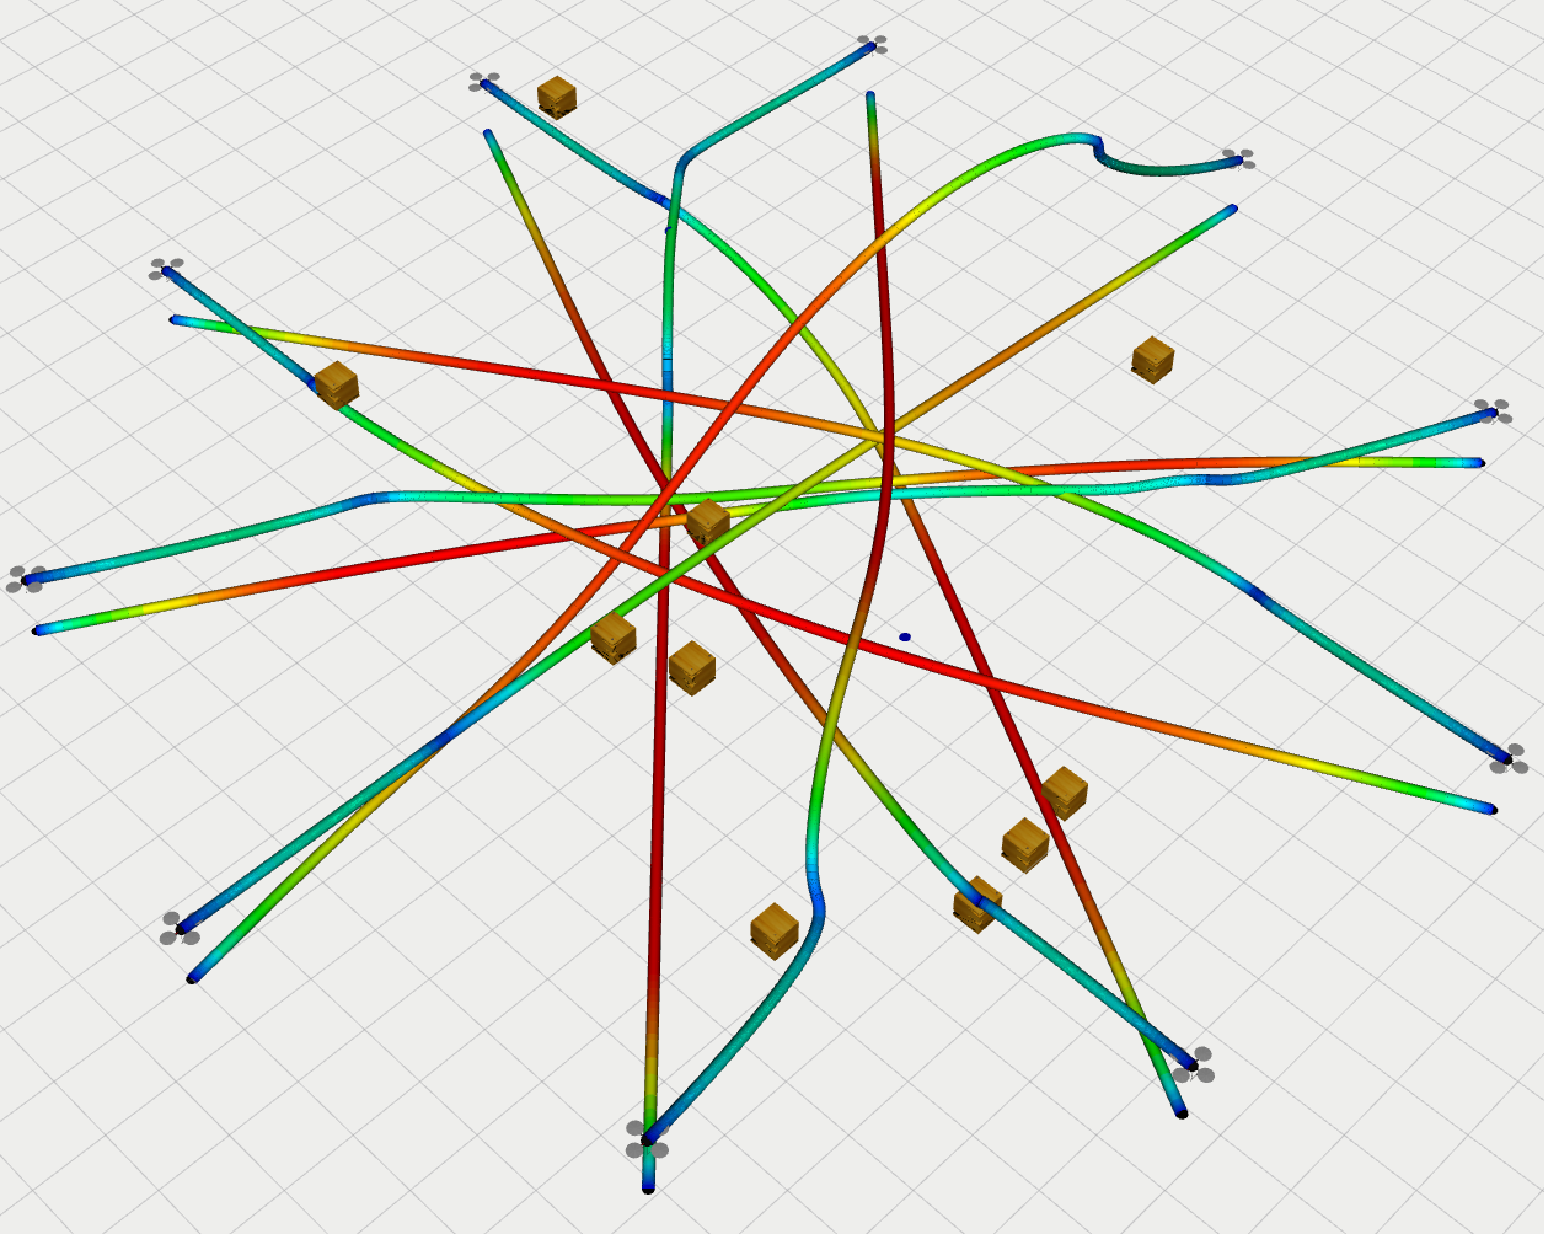
\includegraphics[width=0.45\columnwidth,height=0.14\textheight]{figures/rmader_obs_orbitview.pdf}}
    \hspace{1em}
    \subfloat[Top view]{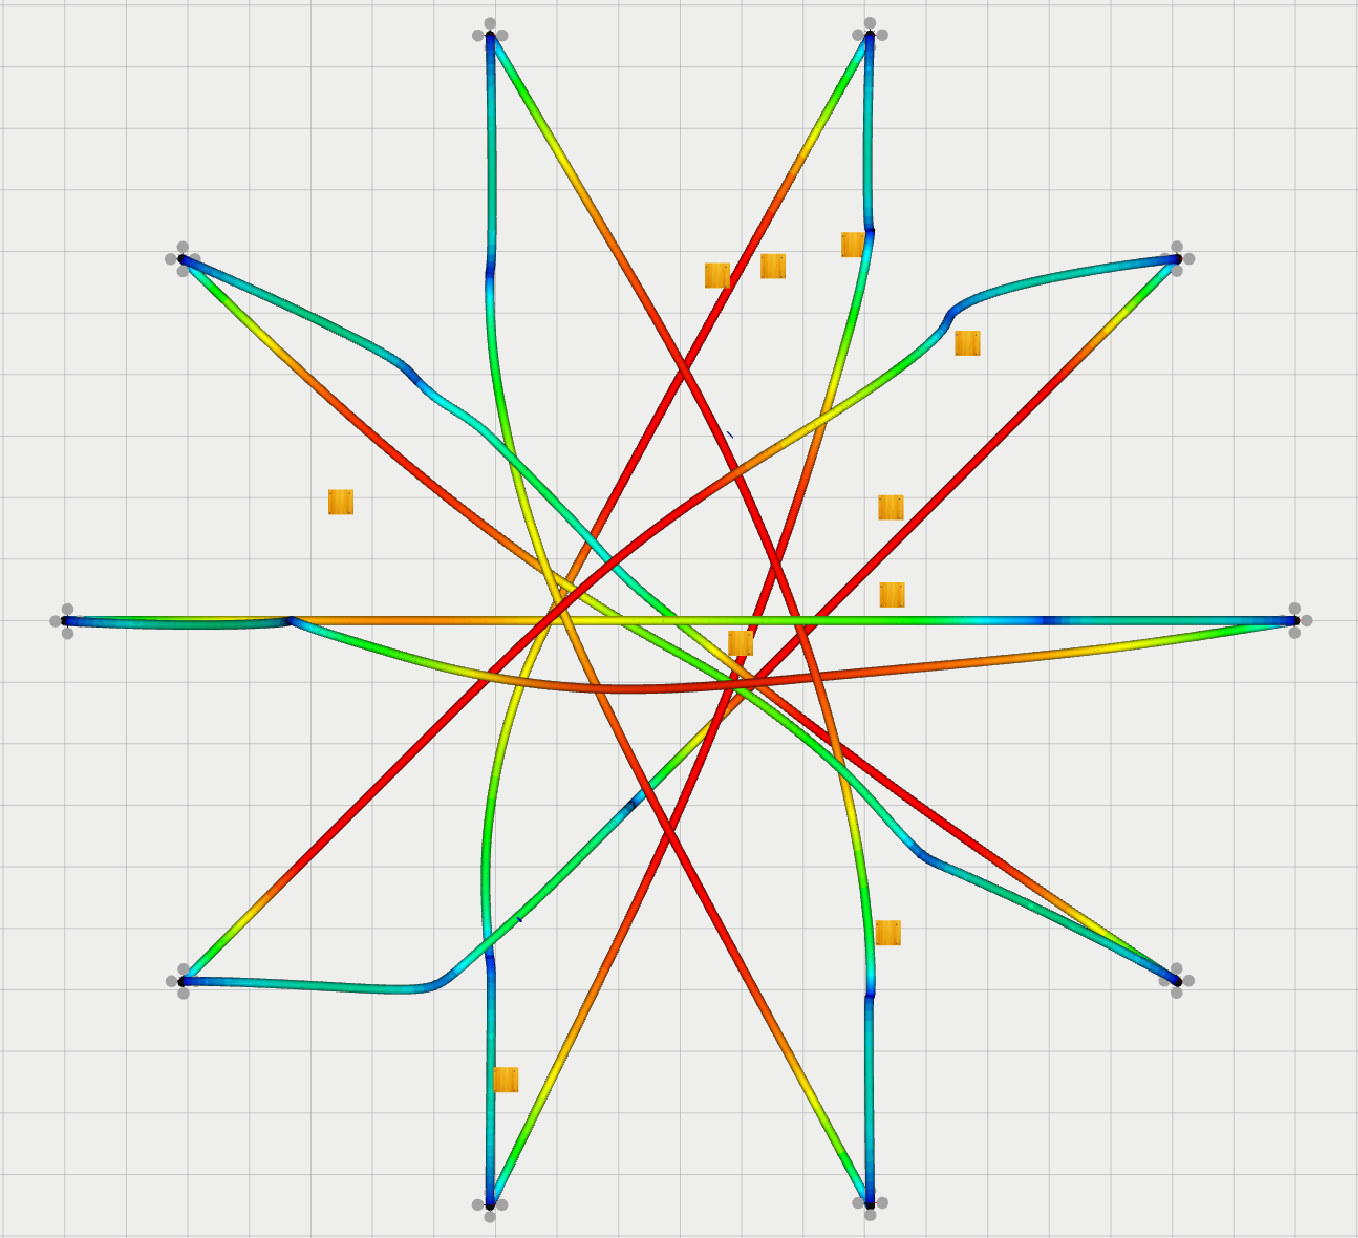
\includegraphics[width=0.45\columnwidth,height=0.14\textheight]{figures/rmader_obs_topview.pdf}}
    \caption{\centering 10 RMADER agents with 10 dynamic obstacles - red indicates fast speed and blue shows slow speed}
    \label{fig:rmader_obs}
\end{figure}